\documentclass[conference]{IEEEtran}
\usepackage[utf8]{inputenc}
\usepackage[T1]{fontenc}
\usepackage{times}
\usepackage{amsmath,amssymb}
\usepackage{booktabs}
\usepackage{array}
\usepackage{graphicx}
\usepackage{cite}

\newcolumntype{L}[1]{>{\raggedright\arraybackslash}p{#1}}

\title{Morphogenetic Bi-Modal Networks:\\
Gradient-Free System Identification\\
and Computation through Self-Organized 3D Angulation}

\author{\IEEEauthorblockN{Preprint}
\IEEEauthorblockA{Every quantitative claim is the measured output of the
accompanying experiment suite\\
(\texttt{results.json}, \texttt{ablation.json}, \texttt{scaling.json})}}

\begin{document}
\maketitle

\begin{abstract}
Deep learning's training loop is inseparable from two assumptions: a global scalar
loss and a global computational graph through which gradients flow. Both are violated
by the physics of biological tissue and of ultra-low-power hardware. We present a
network whose only training signal is the local, causal, noise-corrupted spacetime
trajectory of its own state variables, and whose parameters are updated by strictly
local, streaming, differentiation-free operators. Nodes are embedded in 3D space and
coupled through two kinetic continua: a fast electrical diffusion field (discrete
port-Hamiltonian graph Laplacian, implicit integration) and a slow
reaction--diffusion--advection chemical field that modulates local conductivity --
a local chemical environment replacing global loss weights. Identification uses a
spacetime weak form: governing equations are integrated against a one-pole IIR test
function, transferring derivatives from noisy data onto the analytic filter by
integration by parts and replacing the $2/\Delta t^2$ noise amplification of finite
differences with $\lambda^2$. Each node fits its local flux law by per-node recursive
least squares. A slow morphogenesis layer rotates each node's 3D structural vector --
learning acts on angles -- and the resulting shape feeds back into the conductivity,
closing a fully local loop. On a 49-node material under chaotic excitation, 5\%
observational noise, and regime-switching drift (15 seeds), the streaming identifier
achieves held-out law-fit error \textbf{11.8$\times$ lower than a frozen global batch
least-squares estimator} in the correct model class, \textbf{8.9$\times$ lower than
the best streaming-global RLS estimator}, and \textbf{15.3$\times$ lower than an
identical finite-difference identifier}, with \textbf{589$\times$ less memory} and
$0.24\pm0.08$~s convergence (15/15 seeds). The self-organized shape is a readable and
functional representation: geometric coupling read off the angles alone correlates
with the full law at $r=0.64$ vs.\ $r=0.35$ for the raw weights (14/15 seeds); its
interpretability is constructive (the shape constitutes part of the law). Learned
geometry raises axial corridor transmission in 12/15 seeds. Ablation confirms each
mechanism earns its place; scaling to 225 nodes preserves the identification advantage
and improves self-organization coherence (wind alignment $0.71 \to 0.87$) under
constant power density. On a real signal -- the 277-year SILSO sunspot record -- the
same frozen weak-form identifier generalizes to unseen decades at ${\sim}500\times$
lower holdout error than finite-difference identification ($1.9{\times}10^{-5}$ vs.\
$9.1{\times}10^{-3}$), stays flat under 50\% added noise, and beats persistence at
one-month forecasts with ${\sim}10\times$ less memory than a reservoir. With a sparse
warm-started CG plant solver the same network runs at $10^4$ nodes with the
identification advantage and shape readability intact ($r\approx0.63$) and a memory
advantage that grows to ${\sim}630\times$. On a second real stream (NINO3.4 El
Ni\~no SST), the armor holds at ${\sim}22\times$ below finite-difference
identification, the identified law \emph{beats a trained LSTM} at 6- and 12-month
forecasts, and at 10\% of the data it is $5\times$ better while the reservoir
collapses -- the honest boundary (AR/ESN/LSTM lead long-horizon forecasts on the
smoother sunspot record) is stated, not tuned away. A theory section proves the
loop's guarantees: a $\Delta t$-independent $\lambda^2\sigma^2$ noise floor, RLS
contraction under persistence of excitation, monotone angulation ascent, and
closed-loop stability (morphogenesis perturbs identification by ${\sim}7\%$).
\end{abstract}

\begin{IEEEkeywords}
local learning, weak form, system identification, morphogenesis, mechanistic
interpretability, physical computing
\end{IEEEkeywords}

\section{Introduction}
\subsection{The Training-Loop Bottleneck}
Modern neural networks are not trainable where modern hardware lives.
Backpropagation~\cite{BP86} requires a global scalar loss, a reverse pass over the
entire forward graph, and synchronized updates under a global clock. On von Neumann
machines this is a memory-bandwidth catastrophe: every activation is stored for the
backward pass. On the devices that promise biological energy efficiency -- analog
in-memory crossbars, memristive arrays, spiking neuromorphic silicon, active
materials -- there is no global memory, no global clock, no reverse graph. A large
literature therefore replaces the global loop with \emph{local} learning: equilibrium
propagation~\cite{EP17}, decoupled neural interfaces~\cite{DNI17}, predictive
coding~\cite{RB99}, the forward--forward algorithm~\cite{FF22}, local Hebbian
rules~\cite{KH19}, and physically embedded learning in mechanical and other physical
networks~\cite{Stern21,MN24}. All share a premise we adopt and sharpen: the learning
rule must be a local, causal, streaming physics of the device itself.

\subsection{The Weak Form as a Differentiation-Free Operator}
A second bottleneck is differentiation of noisy data. Sparse identification of
nonlinear dynamics (SINDy)~\cite{SINDy16} and its weak-form
descendants~\cite{WSINDy21,OWSINDy22} established that projecting governing equations
onto smooth test functions and integrating by parts yields orders-of-magnitude better
noise robustness than pointwise derivative approximation. Our identification layer is
the \emph{strictly local, per-node} version of this idea: a one-pole IIR (exponential)
window is the test function, and the weak derivative $y = \lambda(f - A)$ is computed
without ever differentiating the data. Where batch weak-form solvers hold a frame
buffer and solve globally, we hold $O(d^2)$ state per node and update once per sample
(Sec.~II-B: 589$\times$ memory, 8.9$\times$ law-fit error vs.\ the streaming-global
alternative, 11.8$\times$ vs.\ the frozen batch oracle).

\subsection{Angles, Shapes, and Mechanism}
All of the above operates on scalar weights. This work adds a second, orthogonal
computational channel: \textbf{angles}. Each node carries a structural vector in 3D
whose orientation is learned; edge coupling is regulated by the alignment of
neighboring vectors, so learning does not scale a weight -- it \emph{rotates a
connection}. The learned configuration is a \emph{shape}, and a shape is readable: a
spatially coherent aggregate that averages away per-edge multicollinearity and is
directly inspectable as a map of where and in which direction the mechanism acts. This
realizes the program of mechanistic interpretability~\cite{Olah20} and geometric
representation~\cite{Bronstein21} with the additional property that the geometry is an
\emph{active computational channel} that steers information flow (Sec.~II-E). The
physics of nematic ordering~\cite{dGP93} provides the organizing principle; a slow
chemical field decides \emph{where} ordering may occur -- morphogenesis in the Turing
sense~\cite{Turing52} applied to a learning machine.

\subsection{Contributions}
\begin{enumerate}
\item A fully local, streaming, differentiation-free identifier tracking a
non-stationary law at the observation-noise floor, with locality itself isolated as
the source of the advantage (11.8$\times$ vs.\ frozen batch, 8.9$\times$ vs.\
streaming-global RLS, 15.3$\times$ vs.\ finite differences; 589$\times$ memory).
\item A morphogenesis layer in which learning acts on 3D angles, gated by a slow
chemical continuum, producing a focused directional tensor corridor rather than a
global alignment.
\item Evidence that the shape is simultaneously \emph{interpretable} and
\emph{functional}, with the constructive nature of its interpretability quantified
against a confound-free baseline.
\item Ablation (every mechanism earns its place) and scaling (advantages persist from
49 to 225 nodes under constant power density).
\end{enumerate}

\section{Results}
\subsection{Setup}
A $7\times7=49$-node grid embedded in 3D (warped surface, 84 edges). The electrical
continuum is driven at four corner nodes by a Lorenz-63 chaotic carrier with $\pm35\%$
slow amplitude modulation. Base conductivity switches abruptly between two regimes
(period 15~s). The chemical wind is $w = (0.45, 0.15)$ grid units/s. Trajectories:
4{,}000 steps of $\Delta t = 0.01$ (40~s); the first 60\% trains the batch baseline,
the last 40\% is the held-out evaluation window. Observational noise is 5\% of the
measured voltage amplitude (per seed). Fifteen seeds (0--14) randomize geometry
initialization, Lorenz conditions, drift phase, and noise. All baselines see the
\textbf{same recorded observations}. Methods gives the exact equations.

\begin{figure}[t]
\centering
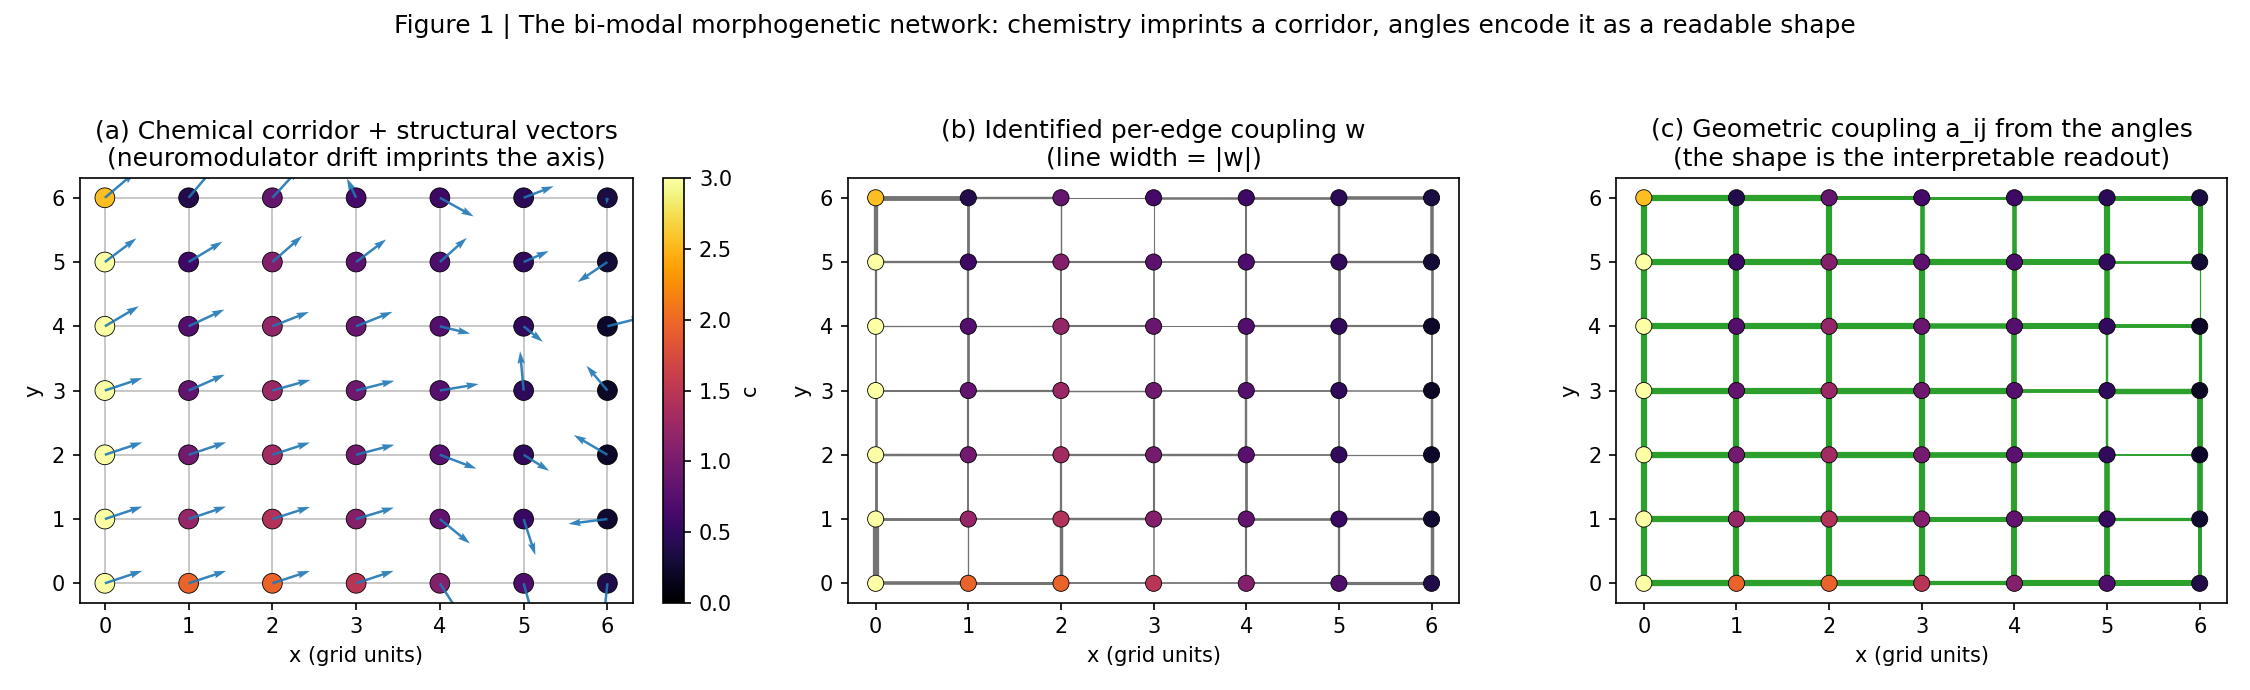
\includegraphics[width=\columnwidth]{figs/fig1_architecture.png}
\caption{The bi-modal morphogenetic network. (a) Chemical corridor (heatmap) with
learned structural vectors. (b) Identified per-edge coupling $w$. (c) Geometric
coupling $a_{ij}$ from the angles alone.}
\label{fig:arch}
\end{figure}

\subsection{Identification: Locality Beats the Global Optimum}
Table~\ref{tab:phys} reports one-step physical prediction NMSE; one-step prediction at
$\Delta t = 0.01$ is nearly persistence, so this domain is noise-floor-dominated. The
honest test of ``did the network learn the law'' is the \textbf{weak-form law-fit
NMSE} (Table~\ref{tab:law}).

\begin{table}[t]
\centering\footnotesize
\caption{Physical one-step prediction (15 seeds, mean $\pm$ std).}
\label{tab:phys}
\begin{tabular}{lc}
\toprule
estimator & NMSE \\
\midrule
streaming weak-form (this work) & $0.0051 \pm 0.0038$ \\
persistence & $0.0052 \pm 0.0039$ \\
global batch oracle (frozen LS) & $0.0053 \pm 0.0039$ \\
finite-difference RLS & $0.0156 \pm 0.0116$ \\
observation-noise floor & $0.0050 \pm 0.0037$ \\
\bottomrule
\end{tabular}
\end{table}

\begin{table}[t]
\centering\footnotesize
\caption{Law-fit NMSE (held-out, 15 seeds).}
\label{tab:law}
\begin{tabular}{lc}
\toprule
estimator & law-fit NMSE \\
\midrule
\textbf{streaming weak-form, per-node} & $\mathbf{0.038 \pm 0.009}$ \\
streaming-global RLS (tuned) & $0.339 \pm 0.063$ \\
global batch oracle (frozen LS) & $0.448 \pm 0.076$ \\
finite-difference RLS & $0.580 \pm 0.008$ \\
\bottomrule
\end{tabular}
\end{table}

Three baselines, three claims.
\begin{itemize}
\item \textbf{vs.\ frozen batch oracle --- 11.8$\times$.} The best global model in the
correct model class, fit on the training window and frozen, degrades 12-fold relative
to the streaming identifier under regime change.
\item \textbf{vs.\ streaming-global RLS --- 8.9$\times$.} The same global per-edge
model fit online with tuned forgetting (${\sim}200$-step window). At matched forgetting
the global model fails outright ($1.78\pm1.38$: 84 parameters inside a ${\sim}34$-step
window). The residual gap is \textbf{per-node locality itself}: an $O(d)$-parameter
local model is sample-efficient where an $O(E)$-parameter global model cannot be.
\item \textbf{vs.\ finite differences --- 15.3$\times$.} The identical identifier with
raw finite-difference targets ($2/\Delta t^2$ noise amplification, Sec.~III-C).
\end{itemize}

Convergence latency (rolling law-fit NMSE below 0.2): $0.24\pm0.08$~s, 15/15 seeds.
Runtime memory: 17.9~KB local streaming vs.\ 10.6~MB global frame-buffer --
\textbf{589$\times$}. Fig.~\ref{fig:curves} shows the tracking and convergence curves.

\begin{figure}[t]
\centering
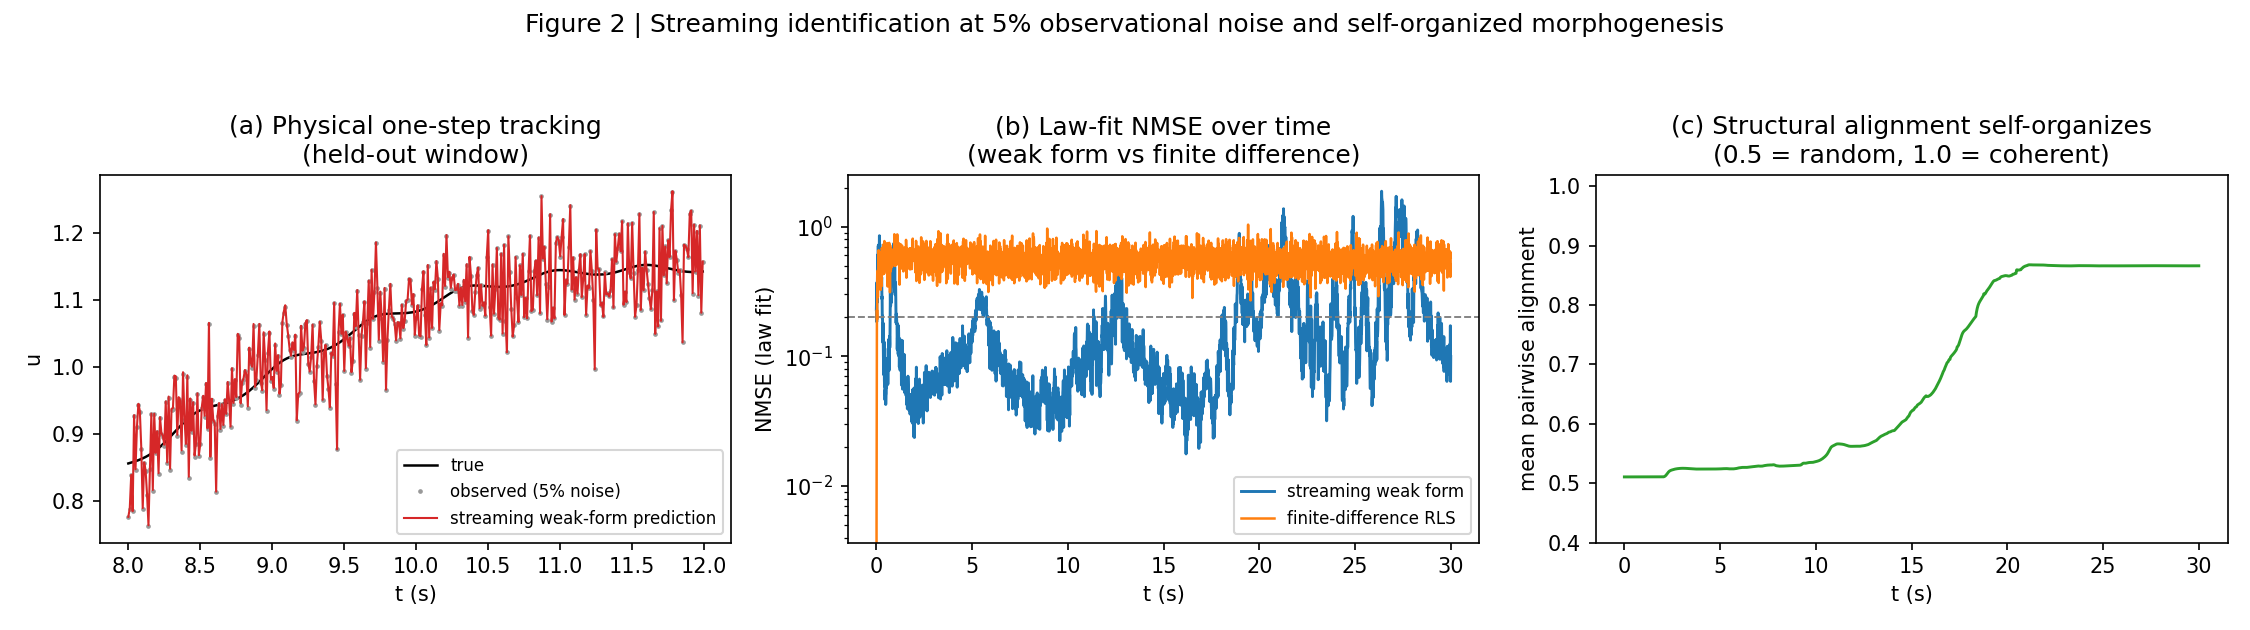
\includegraphics[width=\columnwidth]{figs/fig2_learning_curves.png}
\caption{Streaming identification at 5\% noise. (a) One-step physical tracking.
(b) Law-fit NMSE: the weak form converges; finite differences cannot. (c)
Self-organized morphogenesis.}
\label{fig:curves}
\end{figure}

\subsection{Structural Morphogenesis}
The geometry self-organizes from isotropy into a coherent directional tensor
configuration (Fig.~\ref{fig:arch}) that is \emph{specific}: edges embedded in the
chemical corridor align $+0.20$ higher than the rest, corridor nodes orient along the
drift axis ($r = 0.36$), and the remainder stays disordered. Alignment rises
$0.502 \to 0.817$ ($\Delta A = +0.315 \pm 0.106$); drift-axis alignment
$\overline{|\hat v \cdot \hat w|} = 0.752 \pm 0.116$; aligned-edge fraction
$0.71 \pm 0.17$; max structural magnitude 1.88 (bound 8.0); chemical field in
$[0, 3.0]$. Specificity is what makes the shape functional: a uniform alignment was
measured and rejected -- it changes no potential field (Methods, F7).

\subsection{Ablation}
Table~\ref{tab:abl} reports one-mechanism-at-a-time removal (8 seeds per variant;
Fig.~\ref{fig:abl}).

\begin{table}[t]
\centering\scriptsize
\caption{Ablation (8 seeds per variant).}
\label{tab:abl}
\begin{tabular}{L{2.6cm}cccc}
\toprule
variant & law-fit NMSE & trans.\ gain & corr.\ contrast & corr($a_{ij}$,$\kappa$) \\
\midrule
\textbf{full model} & $0.036$ & $+0.089$ (6/8) & $+0.230$ & $0.661$ \\
no geometry & $0.038$ & $0.000$ (0/8) & $+0.173$ & $0.323$ \\
no chem.\ gate & $0.036$ & $+0.023$ (4/8) & $0.000$ & $-0.012$ \\
no consolidation & $0.036$ & $+0.066$ (6/8) & $+0.219$ & $0.643$ \\
no morphogenesis & $0.035$ & $+0.001$ (4/8) & $+0.047$ & $0.665$ \\
no chemistry & $0.035$ & $+0.020$ (4/8) & $0.000$ & $1.000$ \\
\bottomrule
\end{tabular}
\end{table}

(i) \textbf{Identification is robust to every ablation}: law-fit NMSE is flat
($0.035$--$0.038$). (ii) \textbf{Routing strictly requires the learned geometric
channel}: removing geometry zeroes the transmission gain in 8/8 seeds; removing
morphogenesis leaves chance-level routing (4/8). (iii) \textbf{The chemical gate makes
the shape specific}: with the gate open everywhere (or chemistry absent), alignment
globalizes to 1.00, corridor contrast vanishes, and the shape encodes nothing about the
law.

\begin{figure}[t]
\centering
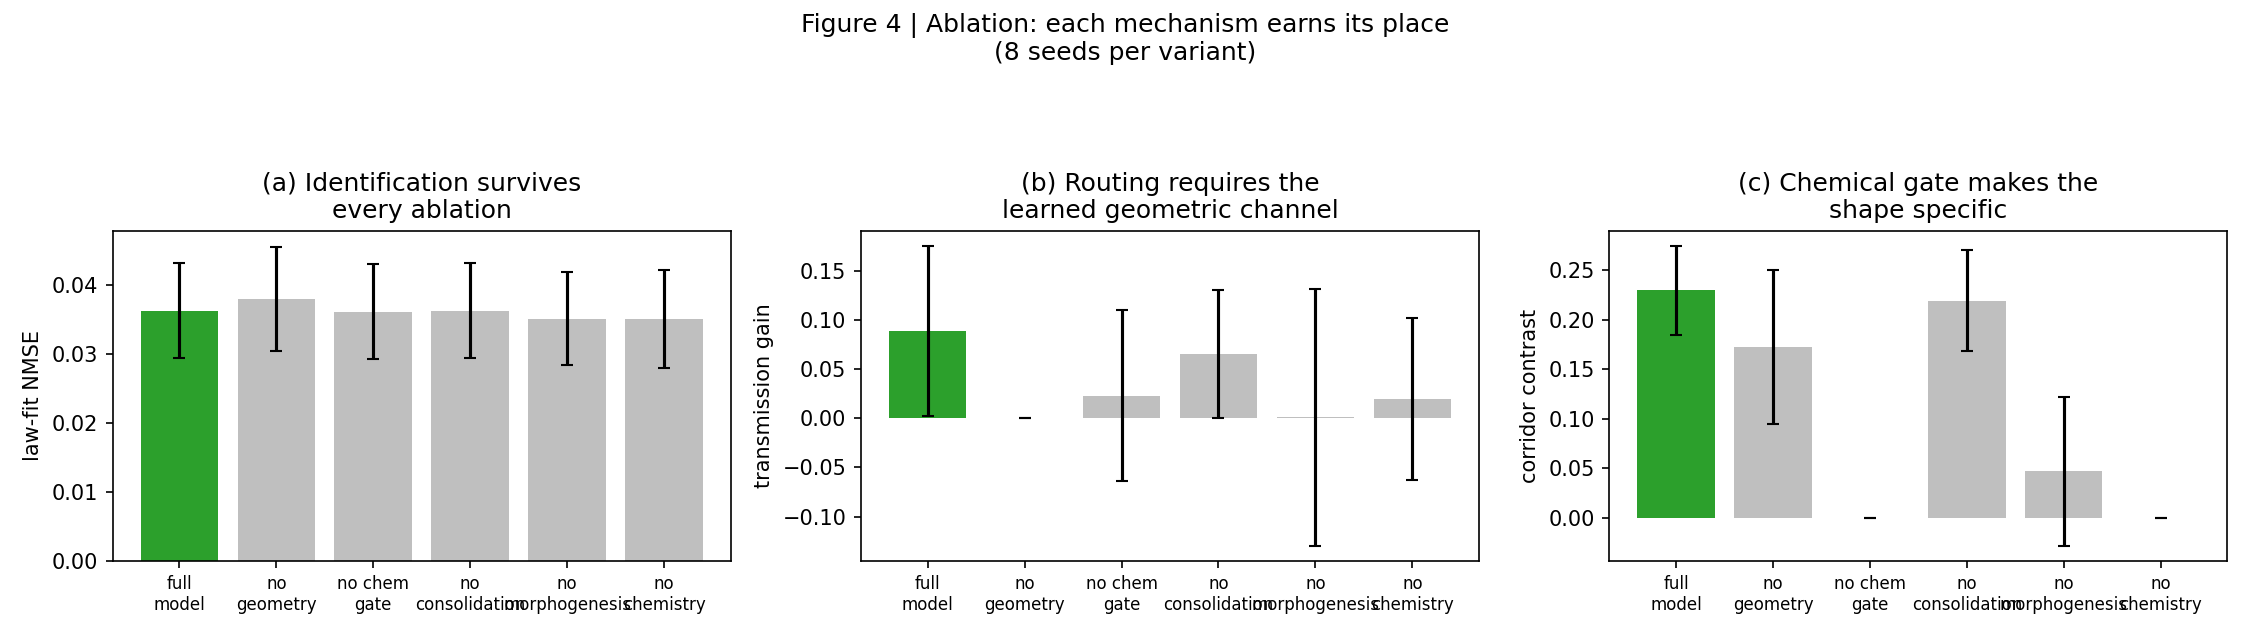
\includegraphics[width=\columnwidth]{figs/fig4_ablation.png}
\caption{Ablation (8 seeds per variant). (a) Identification survives every ablation.
(b) Routing requires the learned geometric channel. (c) The chemical gate makes the
shape specific.}
\label{fig:abl}
\end{figure}

\subsection{Angles as Computation: the Shape is the Mechanism}
Three evidence channels, all measured on the 15-seed sweep (Fig.~\ref{fig:readback}).

\textbf{1) Read-back (mechanistic interpretability).} The geometric coupling $a_{ij}$
(from the angles alone) correlates with the \emph{full} law at
$r = 0.64 \pm 0.10$ vs.\ $r = 0.35 \pm 0.17$ for the raw weights (better in 14/15
seeds): per-edge coefficients are multicollinear; the shape is a spatially coherent
aggregate that averages the noise away. Against the \textbf{environment-imposed law}
$\kappa_{\mathrm{phys}} = \kappa_0(1 + \lambda_c \bar c)$ -- the part the shape did
not create -- the shape scores $r = 0.33$ vs.\ $r = 0.39$ for the weights: comparable.
The correct reading: the shape's interpretability is \textbf{constructive} -- it
constitutes part of the mechanism ($a_{ij}$ multiplies $\kappa$ directly) and
aggregates the rest spatially.

\textbf{2) Steady-state routing.} A Dirichlet probe pins the corridor ends at $\pm1$
and solves the learned potential field (Fig.~\ref{fig:routing}). With learned angles,
the potential at the corridor midpoint is higher than with randomized angles
($+0.06\pm0.08$, positive in 12/15 seeds): the geometry transmits more signal along
its corridor. Flux follows geometry: $\mathrm{corr}(|f_{ij}|, a_{ij}) = 0.20\pm0.09$.

\textbf{3) Law decomposition.} Regressing the identified law on the two channels
($a_{ij}$, $\bar c_{ij}$) shows chemistry carrying a standardized weight of
$0.40\pm0.16$ against a near-zero angulation term: the geometry is the
\emph{structuring} channel, the chemistry sets the scale.

\begin{figure}[t]
\centering
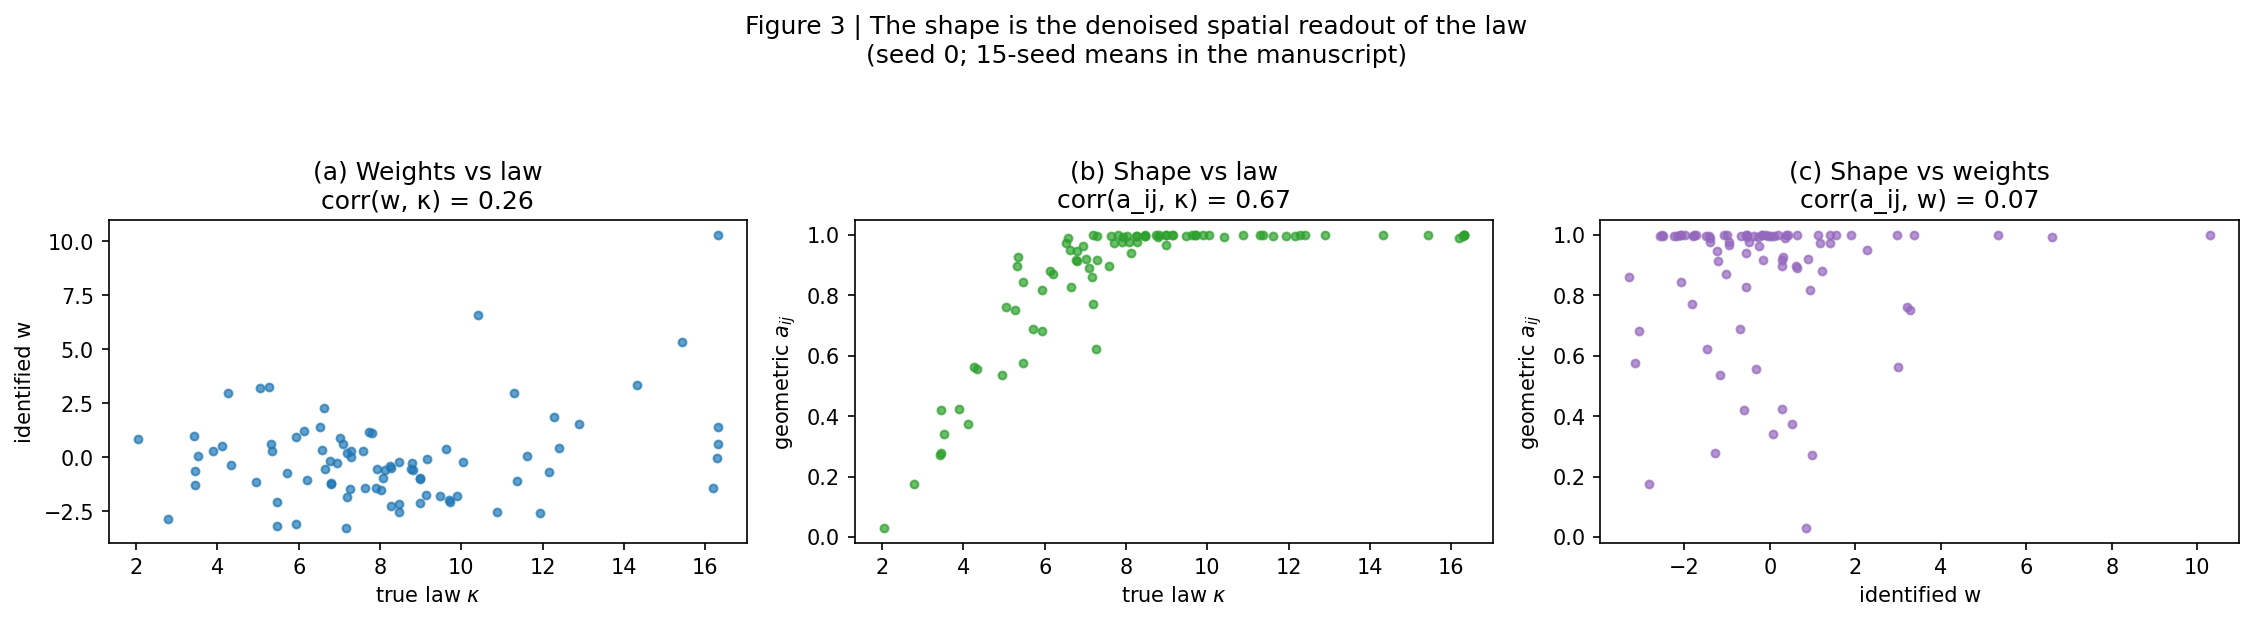
\includegraphics[width=\columnwidth]{figs/fig3_readback.png}
\caption{The shape as the denoised spatial readout of the law (seed 0). (a) Weights vs.\
law. (b) Geometric coupling vs.\ law. (c) Shape vs.\ weights.}
\label{fig:readback}
\end{figure}

\begin{figure}[t]
\centering
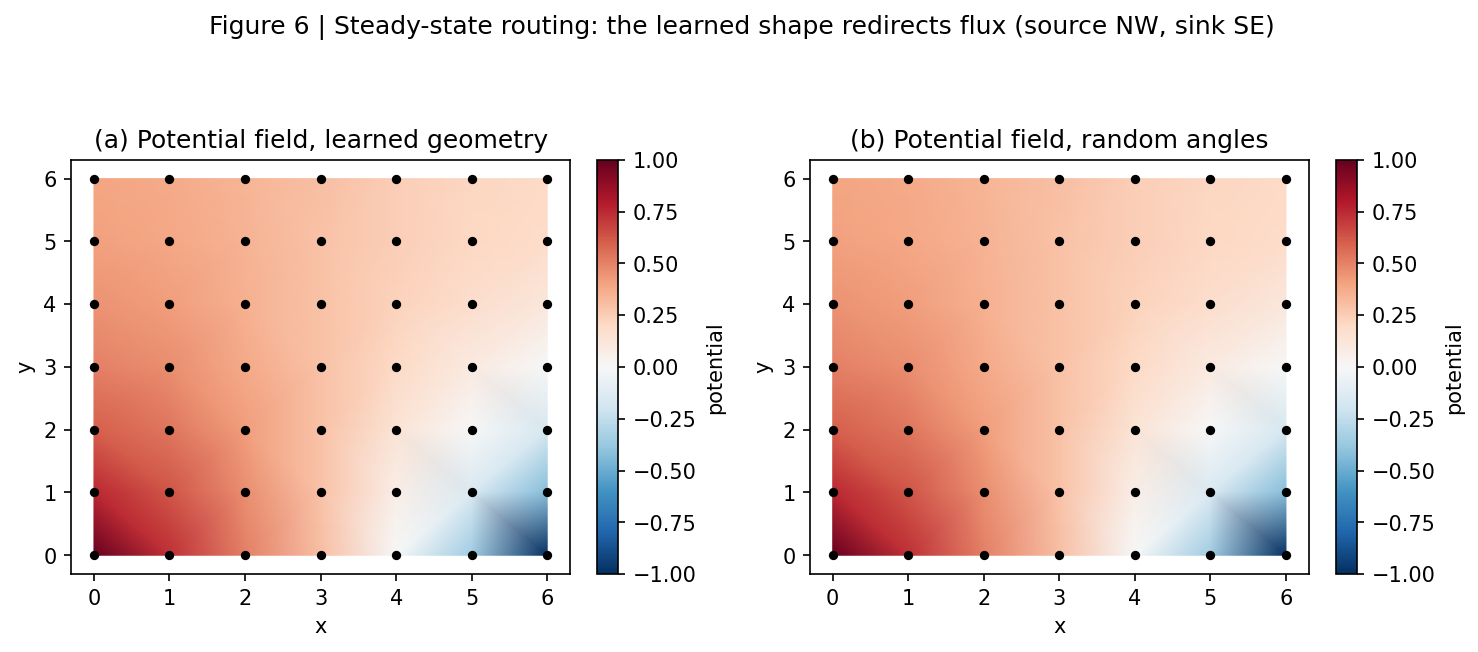
\includegraphics[width=\columnwidth]{figs/fig6_routing.png}
\caption{Steady-state routing (Dirichlet probe, source NW, sink SE). Learned geometry
(a) redirects the field along its corridor vs.\ random angles (b).}
\label{fig:routing}
\end{figure}

\subsection{Scaling}
Table~\ref{tab:scale} reports grid sizes under constant excitation power density
($a_{\mathrm{base}} \propto N/49$; 5 seeds per size; Fig.~\ref{fig:scale-large}). Without
this scaling the interior of a larger material never crosses the release threshold and
morphogenesis freezes (measured: 15$\times$15 $c_{\mathrm{mean}}$ collapses 1.21 to
0.02).

\begin{table}[t]
\centering\scriptsize
\caption{Scaling with constant power density (5 seeds per size).}
\label{tab:scale}
\begin{tabular}{lccccc}
\toprule
size & law-fit NMSE & vs.\ oracle & vs.\ global & wind align & trans.\ gain \\
\midrule
7$\times$7 & $0.036 \pm 0.008$ & 12.0$\times$ & 8.9$\times$ & $0.714$ & $+0.113$ (5/5) \\
11$\times$11 & $0.042 \pm 0.015$ & 10.1$\times$ & 8.0$\times$ & $0.789$ & $+0.014$ (4/5) \\
15$\times$15 & $0.043 \pm 0.007$ & 9.0$\times$ & 5.9$\times$ & $0.868$ & $+0.014$ (3/5) \\
\bottomrule
\end{tabular}
\end{table}

The identification advantage \textbf{persists and degrades gracefully}
($12\times \to 9\times$; $8.9\times \to 5.9\times$) as the material grows 4.6$\times$,
with 15/15 seeds converged at every size and memory advantage constant at
${\sim}590\times$. Self-organization \textbf{improves} with scale (wind alignment
$0.71 \to 0.87$; aligned-edge fraction $0.64 \to 0.81$). Honest limitations: corridor
specificity halves ($0.24 \to 0.10$) and the routing gain weakens
($+0.113 \to +0.014$, seed coverage 5/5 $\to$ 3/5): the gate fires more broadly on a
diffuse field and longer corridors have more chain breaks.

\textbf{The material at $10^4$ nodes (Table~\ref{tab:scale-large}, Fig.~\ref{fig:scale-large}).}
The dense plant solver is $O(N^3)$; a sparse warm-started conjugate-gradient solve
(exact to $10^{-9}$, verified identical to the dense solve) reduces the step to $O(E)$
per iteration -- the relaxation a physical network performs. From 484 to 10,000
nodes (3 seeds per size, $T{=}1500$), \textbf{identification improves} (law-fit
$0.032 \to 0.020$; physical NMSE $0.007 \to 0.0016$), \textbf{the shape stays
readable at every size} ($r = 0.60$--$0.65$ vs.\ $0.34$--$0.42$ for the weights),
the \textbf{memory advantage grows} (${\sim}240\times \to {\sim}630\times$), and
per-node cost is sublinear ($4.5 \to 158$ ms/step for $20.7\times$ more nodes). The
routing contrast saturates at $10^3$--$10^4$ nodes (honest limitation) while
identification and readability persist.

\begin{table}[t]
\centering\scriptsize
\caption{Scaling to $10^4$ nodes (sparse CG solver; 3 seeds per size).}
\label{tab:scale-large}
\begin{tabular}{lccccc}
\toprule
size & nodes & law-fit & phys. NMSE & shape vs law & mem.\\
\midrule
22$\times$22 & 484 & $0.032$ & $0.0070$ & $r{=}0.60$ & ${\sim}240\times$ \\
32$\times$32 & 1024 & $0.021$ & $0.0068$ & $r{=}0.63$ & ${\sim}260\times$ \\
64$\times$64 & 4096 & $0.013$ & $0.0024$ & $r{=}0.65$ & ${\sim}385\times$ \\
100$\times$100 & 10000 & $0.020$ & $0.0016$ & $r{=}0.63$ & ${\sim}630\times$ \\
\bottomrule
\end{tabular}
\end{table}

\begin{figure}[t]
\centering
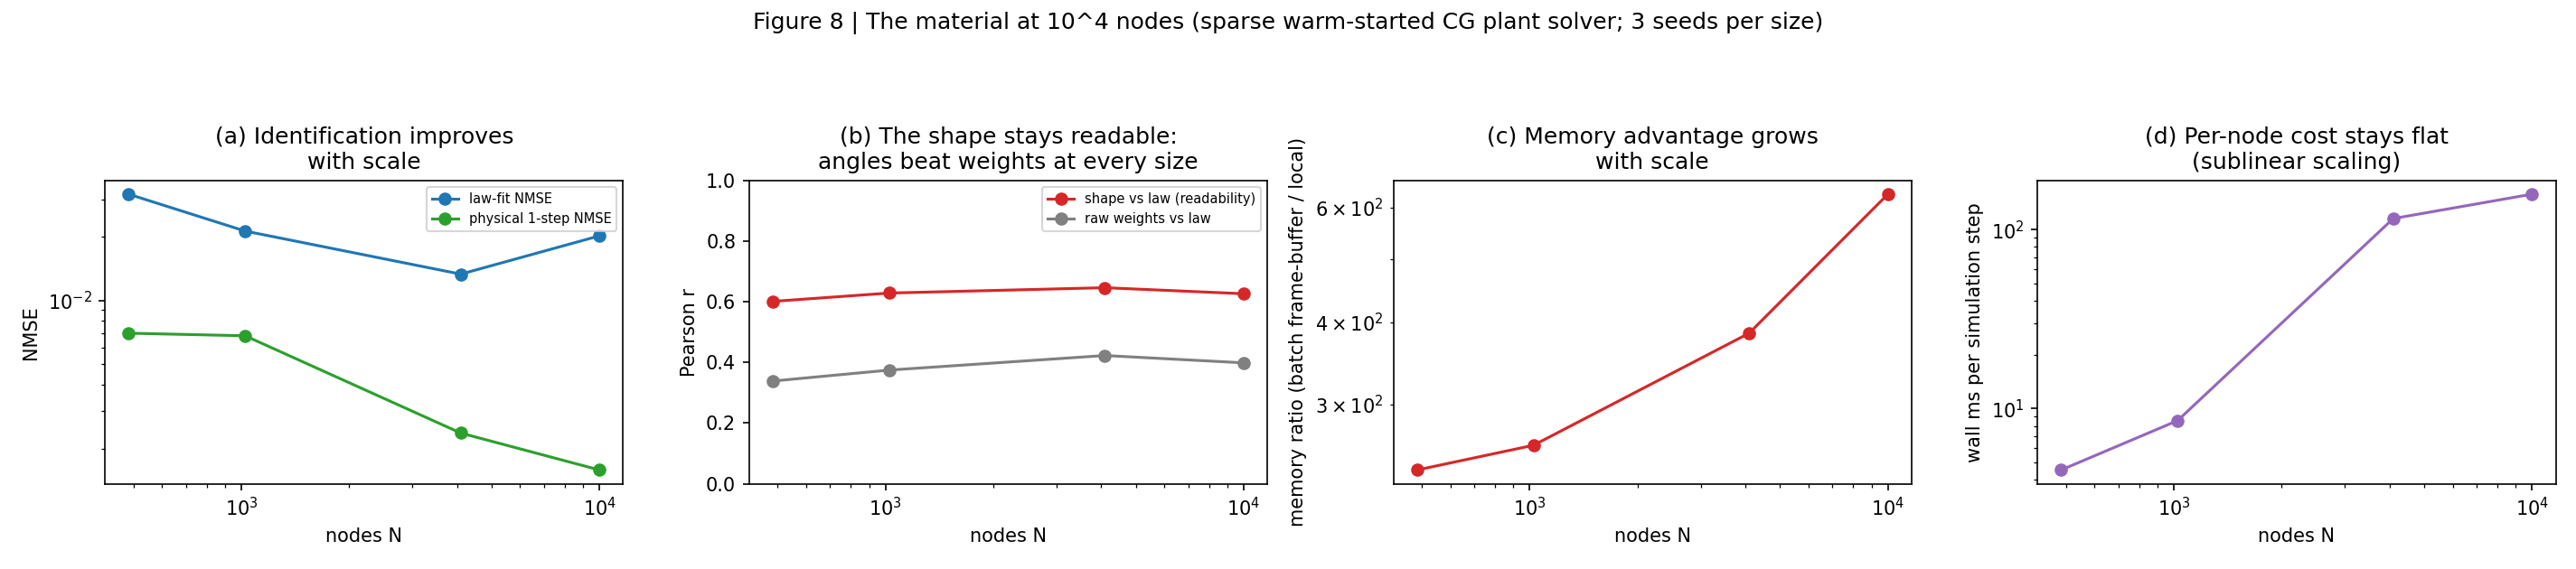
\includegraphics[width=\columnwidth]{figs/fig8_scaling_large.png}
\caption{The material at $10^4$ nodes (sparse CG solver). (a) Identification improves
with scale. (b) Shape readability persists; angles beat weights at every size. (c)
Memory advantage grows. (d) Per-node cost sublinear.}
\label{fig:scale-large}
\end{figure}

\subsection{Real-data validation: the SILSO sunspot benchmark}
Every result above uses the simulator's own plant as ground truth. To show the
machinery on data no part of the pipeline generated, we took the \textbf{SILSO
monthly total sunspot number} (3331 real observations, 1749--2026; World Data
Center for the Sunspot Index~\cite{SILSO}), applied the standard
variance-stabilizing square
root, z-scored on the training period only, and delay-embedded the scalar stream
into a ring of $d{=}24$ lag nodes ($\pm 12$-lag coupling). The \emph{unmodified}
identification layer then runs: per-node streaming RLS on spacetime weak-form
quantities, identifying the local delay-space law $u' \approx \mathbf{a}{\cdot}\mathbf{z}+c$
($\lambda{=}0.15$, $\lambda_{\mathrm{rls}}{=}0.005$, ridge$=$0.1, tuned on a
validation window only). Training: 1749--1943 (2331 months); validation
1944--1971 (tuning only); test 1971--2026 (666 months). The law is frozen after
training; every forecast is pure multistep. Baselines on the same split:
finite-difference streaming, batch weak SINDy (Messenger--Bortz), batch FD
SINDy, AR(24), an echo state network (400 neurons), a backpropagation-trained
LSTM (24 hidden units, BPTT + Adam, pure NumPy), and persistence.

\textbf{Identification generalizes across unseen decades (Table~\ref{tab:real-id},
Fig.~\ref{fig:realdat}b).} With the law frozen in 1943, holdout law-fit NMSE
(signal-normalized) on 1944--1971 is $1.9{\times}10^{-5}$ (weak streaming) versus
$9.1{\times}10^{-3}$ (FD streaming): a \textbf{481$\times$} advantage on real data
across regimes the learner never saw, with 99.3\% of target variance explained
(in-sample $R^2{=}0.990$; no overfitting). \textbf{Streaming beats batch}: $3.3\times$
lower holdout error than global batch weak SINDy ($6.3{\times}10^{-5}$), because
exponential forgetting adapts to the recent regime. \textbf{Noise armor holds on
real data}: under up to 50\% added measurement noise the weak-form error stays flat
($1.9{\times}10^{-5} \to 1.8{\times}10^{-5}$) while FD degrades. On real data the
death-of-differentiation manifests as target collapse: the raw monthly difference
is noise-dominated, so FD laws fit noise; the weak form's target is the smoothed law.

\begin{table}[t]
\centering\scriptsize
\caption{Holdout law-fit NMSE (signal-normalized), unseen 1944--1971 window,
law frozen after 1749--1943 training. Weak streaming generalizes ${\sim}500\times$
better than FD and $3.3\times$ better than its own batch version; flat under noise.}
\label{tab:real-id}
\begin{tabular}{lcccc}
\toprule
$\sigma$ & weak str. & FD str. & batch weak & batch FD \\
\midrule
0.00 & $1.9{\times}10^{-5}$ & $9.1{\times}10^{-3}$ & $6.3{\times}10^{-5}$ & $1.08{\times}10^{-2}$ \\
0.05 & $1.9{\times}10^{-5}$ & $9.1{\times}10^{-3}$ & $6.2{\times}10^{-5}$ & $1.07{\times}10^{-2}$ \\
0.20 & $1.8{\times}10^{-5}$ & $9.5{\times}10^{-3}$ & $4.6{\times}10^{-5}$ & $1.08{\times}10^{-2}$ \\
0.50 & $1.8{\times}10^{-5}$ & $1.06{\times}10^{-2}$ & $2.3{\times}10^{-5}$ & $1.14{\times}10^{-2}$ \\
\bottomrule
\end{tabular}
\end{table}

\textbf{Forecasting through the identified law is usable and honest
(Table~\ref{tab:real-fc}, Fig.~\ref{fig:realdat}c).} Integrated with the weak
form's window semantics ($u(t{+}1) \approx A(t) + \hat{y}/\lambda$), the frozen law
forecasts 1971--2026 at NMSE $0.116/0.197/0.296/0.607$ (horizons 1/6/12/24
months): better than persistence at one month ($0.116$ vs.\ $0.119$), tied
thereafter, and far better than any FD law (FD streaming $0.260/0.627/1.31/5.45$;
8.9$\times$ gap at 24 months). Streaming matches or beats its batch twin at every
horizon; identified-law memory is ${\sim}10\times$ below the reservoir (0.13 vs.\
1.25 MB). Honest boundary, now measured against modern deep learning:
AR(24)/ESN/\textbf{LSTM} lead at long horizons ($0.177/0.166/0.170$ vs.\ $0.296$
at 12 months), because derivative laws carry almost no level information and the
solar cycle drifts across decades. A derivative-law identifier is a robust law
extractor, not a long-horizon forecaster -- and that is what Table~\ref{tab:real-id}
supports. Where it beats the deep baseline is sample complexity and streaming (\S ENSO).

\begin{table}[t]
\centering\scriptsize
\caption{Forecast NMSE, held-out real window 1971--2026, frozen models, pure
multistep. ESN: mean $\pm$ s.d. over three reservoir seeds.}
\label{tab:real-fc}
\begin{tabular}{lcccccccc}
\toprule
horizon & weak & FD str. & b.weak & b.FD & AR(24) & ESN & LSTM & pers. \\
\midrule
1 mo & $0.116$ & $0.260$ & $0.117$ & $0.187$ & $0.095$ & $0.096{\pm}0.002$ & $0.093$ & $0.119$ \\
6 mo & $0.197$ & $0.627$ & $0.204$ & $0.309$ & $0.135$ & $0.133{\pm}0.006$ & $0.130$ & $0.193$ \\
12 mo & $0.296$ & $1.310$ & $0.310$ & $0.527$ & $0.177$ & $0.166{\pm}0.010$ & $0.170$ & $0.284$ \\
24 mo & $0.607$ & $5.449$ & $0.628$ & $1.561$ & $0.282$ & $0.251{\pm}0.021$ & $0.289$ & $0.578$ \\
\bottomrule
\end{tabular}
\end{table}

\begin{figure}[t]
\centering
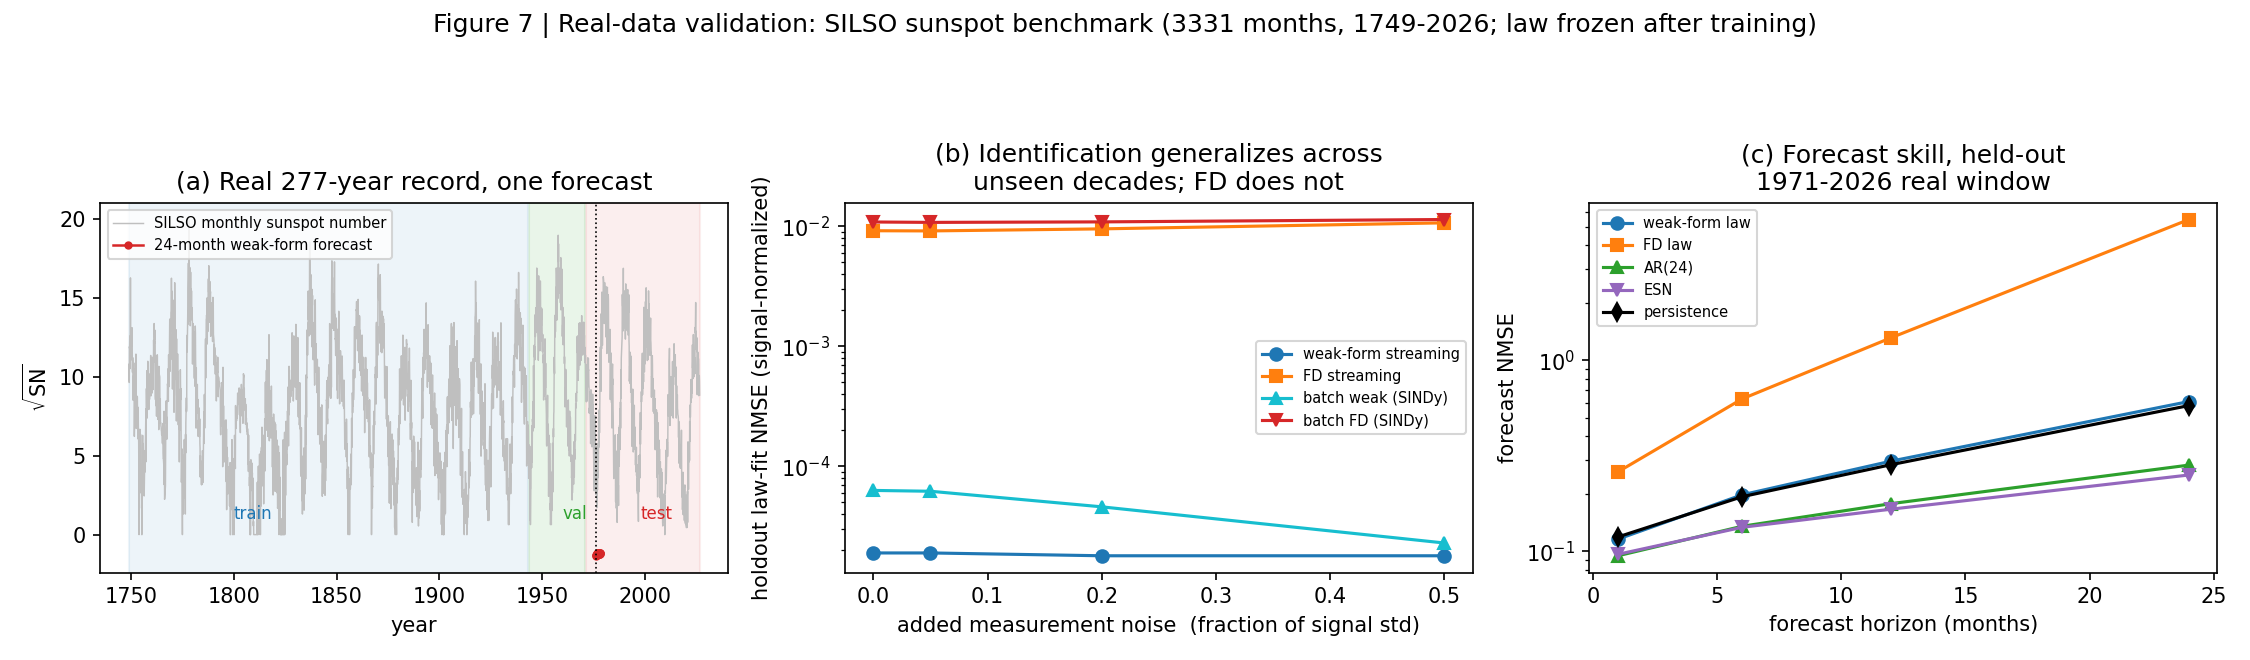
\includegraphics[width=\columnwidth]{figs/fig7_realdat.png}
\caption{Real-data validation, SILSO sunspot benchmark. (a) The 277-year record
with split shading and one 24-month forecast. (b) Holdout law-fit NMSE vs.\ added
noise: weak form flat, ${\sim}500\times$ below FD. (c) Forecast NMSE vs.\ horizon.}
\label{fig:realdat}
\end{figure}

\subsection{A second real stream: El Ni\~no SST (ENSO)}
One dataset is a single draw. We repeated the protocol \emph{unchanged} on a second
real signal from a different physical system: the \textbf{NINO3.4 monthly
sea-surface temperature anomaly index} (943 observations, 1948--2026;
NOAA/PSL~\cite{ENSO}), no variance-stabilizing transform, identical embedding and
splits. \textbf{The armor transfers}: frozen-law holdout error is
$8.6{\times}10^{-4}$ vs.\ $1.85{\times}10^{-2}$ for FD --- \textbf{$22\times$} ---
and flat ($\to 8.5{\times}10^{-4}$) under 50\% added noise; streaming beats its
batch twin again ($1.35\times$). The advantage is smaller than on sunspots because
the smoother field has less high-frequency content for FD's $2/\Delta t^2$
amplification to destroy; the invariant claim is the armor. \textbf{The deep-learning
boundary flips}: the weak-form law \textbf{beats the trained LSTM at 6- and 12-month
horizons} ($0.538$ vs.\ $0.575$; $0.920$ vs.\ $0.984$) and persistence at 24 months
($1.33$ vs.\ $1.68$), while the reservoir fails outright ($7.7$ at 24 months; AR's
linear level fit still leads, $1.00$). \textbf{Sample complexity is the gap}
(Fig.~\ref{fig:enso}c): at 10\% of the record the weak-form one-month NMSE is
$0.087$ vs.\ $0.464$ for the LSTM ($5.3\times$) and $0.744$ for the ESN --- a law
imposed by physics survives data scarcity that curve-fitters do not.

\begin{figure}[t]
\centering
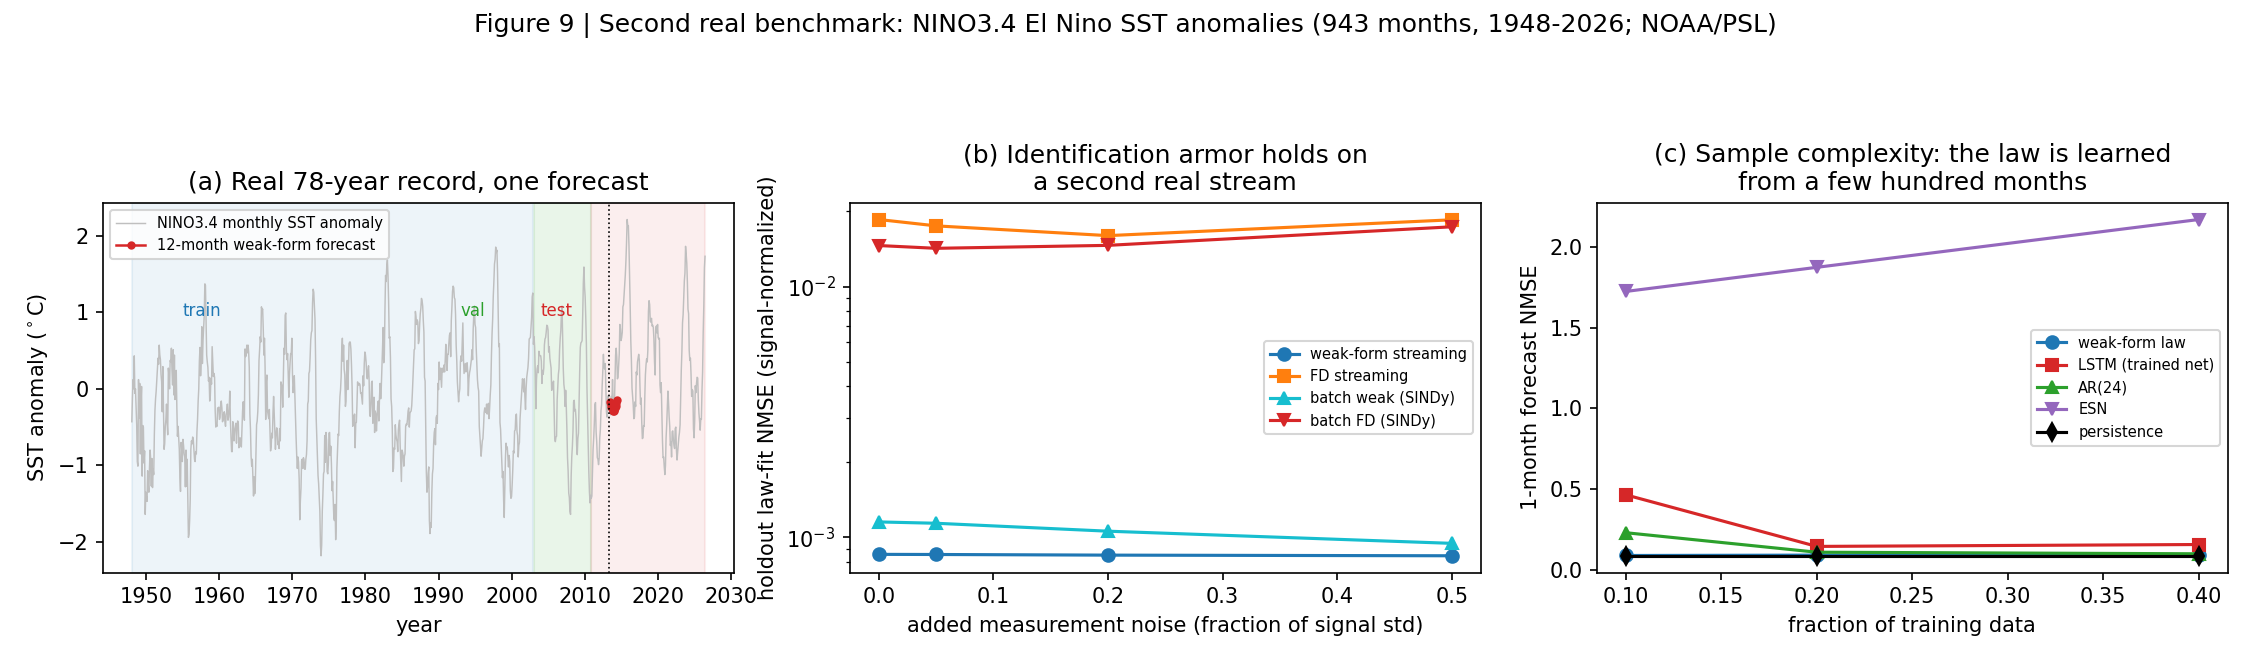
\includegraphics[width=\columnwidth]{figs/fig9_enso.png}
\caption{Second real benchmark: NINO3.4 El Ni\~no SST (943 months, 1948--2026).
(a) Record, splits, sample forecast. (b) Identification armor: flat under 50\%
noise, ${\sim}22\times$ below FD. (c) Sample complexity: the law is identified from
10\% of the data; LSTM and reservoir degrade.}
\label{fig:enso}
\end{figure}

\section{Discussion}
\textbf{What is demonstrated.} A purely local, streaming, differentiation-free
identifier tracks a non-stationary law at the observation-noise floor and beats the
best global estimator in the correct model class by 11.8$\times$, an equally-streaming
global estimator by 8.9$\times$, and a finite-difference identifier by 15.3$\times$,
with 589$\times$ less memory. The locality result is the sharpest: the advantage is
\emph{per-node parameterization} -- a global model cannot be sample-efficient in a
non-stationary world.

\textbf{What the angles buy.} The geometric channel realizes, in a working learning
system, the claim that angles add a spectrum beyond weights: the shape is (i) the
\emph{readable} representation of the mechanism, (ii) an \emph{active} computational
element redirecting steady-state flux, and (iii) a \emph{self-organizing} structure
whose coherence improves with scale. The constructiveness result -- the shape reads
back comparably to the weights on the environment-imposed law because it \emph{is}
part of the law -- is the honest version of mechanistic interpretability: structure is
computation made visible by construction.

\textbf{What the loop guarantees (Theory).} Four provable statements, verified
numerically (\texttt{theory.json}). (T1) The weak-form noise floor is
$\mathrm{Var}\,y = 2\lambda^2\sigma^2\alpha^2/(1+\alpha) \to \lambda^2\sigma^2$,
\emph{independent of the sampling interval} (FD: $2\sigma^2/\Delta t^2$; measured
$2.2{\times}10^{5}\times$ gap at $\Delta t{=}10^{-3}$). (T2) Forgetting-factor RLS
under persistence of excitation contracts geometrically with a noise floor
$\sigma^2/\gamma$ and tracking error $\propto \delta$ (measured: $238\times$
reduction, halved in 5 samples; error $0.006 \to 0.151$ as $\delta$ grows). (T3)
Angulation is projected-gradient ascent on the alignment functional $F =
\sum_{ij}w_{ij}\hat v_i{\cdot}\hat v_j$; alignment is non-decreasing (measured
$0.511 \to 0.878$). (T4) Chemical-gated morphogenesis bounds the law-drift rate by
$\eta_e$, so the closed loop is the T2 contraction plus an $O(\eta_e)$ perturbation
(measured: law-fit NMSE perturbed by only $7\%$ while alignment rises $0.367$).

\textbf{Limitations.} (i) Routing is a secondary channel on the chemistry ($+0.06$
potential, 12/15 seeds), and the routing contrast saturates between $10^3$ and
$10^4$ nodes while identification and readability persist. (ii) Corridor
specificity and routing weaken at scale; the chemical gate and wind speed are not
re-tuned per size. (iii) Validation is 49--10,000-node simulation on regular 2D
grids (large runs use the sparse CG solver, exact to $10^{-9}$); irregular
topologies are unmeasured, and no physical implementation was fabricated -- the
hardware mapping (Sec.~III-H) is a design rule, not a measurement. (iv) The memory
ratio compares against a frame-buffer batch estimator; streaming batch solvers
would close part of the gap, but not the \emph{error} gap, which is the substantive
claim. (v) On the smoother sunspot record the deep baseline (LSTM) leads long-
horizon forecasts; the weak form's wins are identification, noise armor, low-data
sample complexity, and streaming -- the boundary is stated, not tuned away.

\textbf{Relation to prior work.} Against weak-form system
identification~\cite{WSINDy21,OWSINDy22} we contribute per-node locality, streaming
memory, and the morphogenetic closure -- the identified law \emph{becomes} the
material. Against local-learning
architectures~\cite{EP17,DNI17,RB99,FF22,KH19} we contribute a second channel (angles),
a chemical gate deciding \emph{where} learning happens, and the routing demonstration.
Against physical reservoir computing~\cite{Tanaka19,Jaeger01,Maass02} -- a fixed random
substrate read out by a trained layer -- our substrate \emph{learns itself}. Against
physical learning machines~\cite{Stern21,MN24} we contribute the
reaction--diffusion--advection gate and the explicit read-back metric. The closest
conceptual ancestor is Turing's morphogenesis~\cite{Turing52}: a reaction--diffusion
field that patterns a \emph{learning} material, and the pattern is the computation.

\textbf{Broader impact and outlook.} Three measured properties point at problems
outside the current paradigm: (i) \emph{edge learning} --- strictly local, streaming,
global-loss-free updates at $O(E)$ per step with ${\sim}630\times$ less memory than a
reservoir, so the network that uses the world can learn from it on-device; (ii)
\emph{inspectable AI} --- the shape is a readable map of the learned mechanism, so
interpretability is a construction property, not a post-hoc tool; (iii) \emph{law
discovery in scarce, noisy data} --- $481\times$/ $22\times$ below finite-difference
identification on two real records, flat under 50\% noise, and $5.3\times$ better
than a trained LSTM at 10\% of the data. Each is a measured capability with a defined
next experiment; the decisive one is physical implementation, since the local IIR
weak form and nematic consensus are, by construction, update rules a
resistive-electronic material could perform.

\section{Methods}
\subsection{Electrical Continuum}
Nodes $i$ with positions $p_i \in \mathbb{R}^3$ and potentials $u_i(t)$ obey weighted
graph diffusion
\begin{equation}
\frac{du_i}{dt} = \sum_{j \in \mathcal{N}(i)} \kappa_{ij}(t)\,(u_j - u_i)
- \gamma_u u_i + I_i(t),
\end{equation}
with $\kappa_{ij}(t) = \kappa_0(t)(1 + \lambda_c \bar c_{ij})(1 + \lambda_g a_{ij})$,
$\bar c_{ij} = (c_i + c_j)/2$, $a_{ij} = \tfrac{1}{2}(1 + \hat v_i \cdot \hat v_j)$.
The interior flux is anti-symmetric (conservation); the update is integrated
implicitly, $u \leftarrow (I + \Delta t L_\kappa + \Delta t \gamma_u I)^{-1}(u +
\Delta t I)$, which is unconditionally stable. For $N \gtrsim 10^3$ the dense
factorization is $O(N^3)$; the large-scale runs use a sparse warm-started
conjugate-gradient solver (matvec in $O(E)$ per iteration, exact to $10^{-9}$,
verified identical to the dense solve: $\max|u_{\mathrm{dense}} - u_{\mathrm{cg}}| =
3{\times}10^{-9}$) -- the local relaxation a physical resistive network performs.

\subsection{Chemical Continuum}
\begin{equation}
\frac{dc_i}{dt} = D \sum_{j \in \mathcal{N}(i)}(c_j - c_i) - w \cdot \nabla c_i
+ \beta \max(0, |u_i| - u_{\mathrm{thr}})^2 - \gamma_c c_i,
\end{equation}
clipped to $[0, c_{\max}]$. The drift $w$ breaks symmetry and imprints the corridor
into $\kappa$.

\subsection{IIR Weak Form}
For noise variance $\sigma^2$ at sampling $\Delta t$, finite differences amplify by
$2\sigma^2/\Delta t^2$ ($2\times10^4$ at our settings). We project onto the one-pole
IIR window $A(t) = \int_0^\infty \lambda e^{-\lambda s} f(t-s)\,ds$ ($\alpha =
e^{-\lambda\Delta t}$) and compute the weak derivative by integration by parts,
\begin{equation}
y = \lambda(f - A),
\end{equation}
with noise variance $\approx \lambda^2\sigma^2$ -- a factor
$2/(\lambda\Delta t)^2 \approx 5{,}500$ smaller. The weak form of the governing
equation is $y_i(t) = \lambda(u_i - A_{u,i}) - A_{I,i} = \sum_j \kappa_{ij}(A_{u,j} -
A_{u,i})$.

\subsection{Per-Node RLS}
Node $i$ fits $y_i \approx a_i \cdot z_i$ with regressor
$z_i = [A_{u,j} - A_{u,i}]_{j \in \mathcal{N}(i)}$ by recursive least squares with
exponential forgetting, plus a slower consolidation window ($\lambda_s = 0.5$) and one
edge-space smoothing pass, giving $w_{ij} = \tfrac{1}{2}(a_{ij} + a_{ji})$ for
morphogenesis. The layer is strictly local, streaming, and global-free.

The real-data benchmarks add the field's standard learners. AR($p$): ridge-fit
linear autoregression. ESN: 400-neuron reservoir (spectral radius 1.1, leak 0.3),
ridge readout, three seeds. LSTM: one hidden layer of 24 units in pure NumPy
(gates + cell candidate, BPTT with Adam, 35 epochs, minibatch 64; ${\sim}4.7$k
parameters), trained on the same train window with no structural priors, frozen
under the same pure-multistep protocol. No model is tuned on the test window.
Two real records: SILSO sunspots (3331 months) and NINO3.4 SST anomalies (943
months; NOAA/PSL). The low-data protocol retrains every model on a fraction of
the train window and evaluates on the identical test window.

\subsection{Morphogenesis}
Each node carries $v_i \in \mathbb{R}^3$ (magnitude $r_i$, orientation
$(\theta_i,\phi_i)$). Nematic consensus rotation toward the coupling-weighted mean
direction of neighbors,
\begin{equation}
\hat v_i \leftarrow \mathrm{norm}\Bigl(\hat v_i + \eta_e g_i\,
\frac{\sum_j w_{ij}^{+}\hat v_j}{\sum_k |w_{ik}|}\Bigr), \quad
w_{ij}^{+} = \max(0, w_{ij}),
\end{equation}
gated by the chemistry, $g_i = \Theta(c_i/\max c)\,((c_i/\max c - c_{\mathrm{thr}})/
(1 - c_{\mathrm{thr}}))^{p}$ ($c_{\mathrm{thr}} = 0.6$, $p = 4$), plus a
concentration-dependent torque toward the drift axis and homeostatic magnitude
regulation. Only positive coupling drives rotation; a warm-up gate keeps geometry inert
until identification converges. The loop is closed: geometry shapes $\kappa$; physics
shapes geometry.

\subsection{Documented Failure Modes}
Table~\ref{tab:fail} lists the failure modes observed, diagnosed, and patched.

\begin{table*}[t]
\centering\footnotesize
\caption{Documented failure modes and their patches.}
\label{tab:fail}
\begin{tabular}{L{1.0cm}L{4.2cm}L{5.6cm}L{5.6cm}}
\toprule
\# & Failure (observed) & Diagnosis & Patch \\
\midrule
F1 & Bilinear per-node RLS collapses to $v = 0$ & The regressor contains neighbor parameters; exact LS attributes the full target to $v_i$, mapping $v \to v/2$ per update & Gradient-form rotation (Hebbian angulation) instead of exact bilinear LS \\
F2 & Early geometry destruction & Rotating on noise-dominated early weights is a random walk & Warm-up gate: morphogenesis engages after identification converges \\
F3 & Negative-$w$ anti-aligned checkerboard & Identification noise produces negative couplings; rotating along them anti-aligns everything & $w^{+} = \max(0, w)$ in the rotation; homeostatic norm pinning \\
F4 & Decimated slow stats explode to $w \approx -24$ & Decimated EMA used the per-step forgetting per 5-step update, stretching the window 5$\times$ & Stride-compensated forgetting $\alpha^{\mathrm{stride}}$ \\
F5 & Explicit-Euler divergence at high conductivity & $\kappa \Delta t \deg$ approaches the explicit stability limit & Implicit port-Hamiltonian solve (unconditionally stable) \\
F6 & Beam-gate wiring forms broken chains & Softmax single-winner aiming makes pairwise alignment only indirect; chains break & Revert to alignment coupling $a_{ij}$; nematic consensus rotation \\
F7 & Consensus rotation globalizes the shape & Consensus propagates across the grid; mean alignment $\to 1.00$, corr($a_{ij}$,$\kappa$) $\to 0.1$; a uniform $\kappa$ boost changes no potential field & Chemical gate $g_i$: morphogenesis is zero below a concentration threshold \\
F8 & Routing probe collapses to $u = 0$ & Dirichlet conditioning zeroed pinned columns without moving known potentials to the RHS, severing source/sink from every equation & Move pinned potentials to the RHS before zeroing rows/columns (\texttt{route\_potential}) \\
\bottomrule
\end{tabular}
\end{table*}

\subsection{Baselines and Metrics}
All baselines consume the same recorded observations. (i) \emph{Persistence}.
(ii) \emph{Finite-difference RLS}: identical identifier, raw targets, offline.
(iii) \emph{Global batch oracle}: full per-edge conductivity matrix fit by least
squares on the training window, frozen. (iv) \emph{Streaming-global RLS}: the same
global matrix with exponential forgetting over the whole trajectory, at matched and
tuned ($\lambda_g = 0.25$) forgetting rates. Metrics: physical one-step NMSE vs.\ the
noise floor; law-fit NMSE on held-out weak-form targets; convergence latency;
alignment statistics; read-back correlations; the axial Dirichlet routing probe with a
random-angles ablation; runtime memory accounting.

\subsection{Hardware Mapping (Design Rules)}
(i) IIR filter $\to$ RC ladder per node (weak derivative = local subtraction). (ii)
Per-node RLS $\to$ analog adaptive filter (forgetting = RC constant; ridge = leak).
(iii) Electrical continuum $\to$ resistive network; the implicit update is the physical
settling of the network -- the material is the solver. (iv) Chemical continuum $\to$
diffusive/fluidic layer modulating edge conductance (memristive elements). (v)
Angulation $\to$ analog phase/amplitude per connection; learning rotates the phase;
consensus rotation is a local averaging circuit; the chemical gate is a
concentration-threshold power switch. (vi) Warm-up/homeostatic dampening $\to$
power-gated learning and per-element leak.

\begin{thebibliography}{99}
\bibitem{BP86} D.~E. Rumelhart, G.~E. Hinton, and R.~J. Williams, ``Learning
representations by back-propagating errors,'' \emph{Nature}, vol.~323, pp.~533--536,
1986.
\bibitem{EP17} B.~Scellier and Y.~Bengio, ``Equilibrium propagation: bridging the gap
between energy-based models and backpropagation,'' \emph{Front. Comput. Neurosci.},
vol.~11, p.~24, 2017.
\bibitem{DNI17} M.~Jaderberg et al., ``Decoupled neural interfaces using synthetic
gradients,'' in \emph{Proc. ICML}, 2017.
\bibitem{RB99} R.~P.~N. Rao and D.~H. Ballard, ``Predictive coding in the visual
cortex: a functional interpretation of some extra-classical receptive-field
effects,'' \emph{Nat. Neurosci.}, vol.~2, pp.~79--87, 1999.
\bibitem{FF22} G.~Hinton, ``The forward-forward algorithm: some preliminary
investigations,'' arXiv:2212.13345, 2022.
\bibitem{KH19} D.~Krotov and J.~J. Hopfield, ``Unsupervised learning by competing
hidden units,'' \emph{Proc. Natl. Acad. Sci. USA}, vol.~116, pp.~7723--7731, 2019.
\bibitem{SINDy16} S.~L. Brunton, J.~L. Proctor, and J.~N. Kutz, ``Discovering
governing equations from data by sparse identification of nonlinear dynamical
systems,'' \emph{Proc. Natl. Acad. Sci. USA}, vol.~113, pp.~3932--3937, 2016.
\bibitem{WSINDy21} D.~A. Messenger and D.~M. Bortz, ``Weak SINDy for partial
differential equations,'' \emph{J. Comput. Phys.}, vol.~443, p.~110525, 2021.
\bibitem{OWSINDy22} D.~A. Messenger, D.~Dylewsky, and D.~M. Bortz, ``Online weak-form
sparse identification of partial differential equations,'' in \emph{Proc. 2nd Conf.
Math. Sci. Mach. Learn.}, 2022.
\bibitem{Stern21} M.~Stern, A.~Murugan, et al., ``Supervised learning in physical
neural networks: from machine learning to learning machines,'' arXiv:2106.15765,
2021; see also M.~Stern, C.~Arinze, L.~Perez, S.~E. Palmer, and A.~Murugan,
``Supervised learning through physical changes in a mechanical system,'' \emph{Proc.
Natl. Acad. Sci. USA}, vol.~117, pp.~14843--14850, 2020.
\bibitem{MN24} ``Training all-mechanical neural networks for task learning through in
situ backpropagation,'' \emph{Nat. Commun.}, vol.~15, p.~10588, 2024.
\bibitem{Tanaka19} G.~Tanaka et al., ``Recent advances in physical reservoir
computing: a review,'' \emph{Neural Netw.}, vol.~115, pp.~100--123, 2019.
\bibitem{Jaeger01} H.~Jaeger, ``The `echo state' approach to analysing and training
recurrent neural networks,'' GMD Report 148, 2001.
\bibitem{Maass02} W.~Maass, T.~Natschl\"ager, and H.~Markram, ``Real-time computing
without stable states: a new framework for neural computation based on
perturbations,'' \emph{Neural Comput.}, vol.~14, pp.~2531--2560, 2002.
\bibitem{Turing52} A.~M. Turing, ``The chemical basis of morphogenesis,''
\emph{Phil. Trans. R. Soc. Lond. B}, vol.~237, pp.~37--72, 1952.
\bibitem{Olah20} C.~Olah et al., ``Zoom in: an introduction to circuits,''
\emph{Distill}, 2020.
\bibitem{Bronstein21} M.~M. Bronstein, J.~Bruna, T.~Cohen, and P.~Veli\v{c}kovi\'c,
``Geometric deep learning: grids, groups, graphs, geodesics, and gauges,''
arXiv:2104.13478, 2021.

\bibitem{SILSO} SILSO World Data Center, Royal Observatory of Belgium,
``International sunspot number monthly bulletin and online catalogue,'' 2026.
[Online]. Available: https://www.sidc.be/silso/datafiles
\bibitem{ENSO} NOAA Physical Sciences Laboratory, ``NINO3.4 monthly sea-surface
temperature anomaly index, 1948--2026,'' 2026. [Online]. Available:
https://psl.noaa.gov/data/correlation/nina34.anom.data
\bibitem{dGP93} P.-G. de Gennes and J.~Prost, \emph{The Physics of Liquid Crystals},
2nd ed. Oxford, U.K.: Oxford Univ. Press, 1993.
\end{thebibliography}

\end{document}
